% Template for PLoS
% Version 3.6 Aug 2022
%
% % % % % % % % % % % % % % % % % % % % % %
%
% -- IMPORTANT NOTE
%
% This template contains comments intended 
% to minimize problems and delays during our production 
% process. Please follow the template instructions
% whenever possible.
%
% % % % % % % % % % % % % % % % % % % % % % % 
%
% Once your paper is accepted for publication, 
% PLEASE REMOVE ALL TRACKED CHANGES in this file 
% and leave only the final text of your manuscript. 
% PLOS recommends the use of latexdiff to track changes during review, as this will help to maintain a clean tex file.
% Visit https://www.ctan.org/pkg/latexdiff?lang=en for info or contact us at latex@plos.org.
%
%
% There are no restrictions on package use within the LaTeX files except that no packages listed in the template may be deleted.
%
% Please do not include colors or graphics in the text.
%
% The manuscript LaTeX source should be contained within a single file (do not use \input, \externaldocument, or similar commands).
%
% % % % % % % % % % % % % % % % % % % % % % %
%
% -- FIGURES AND TABLES
%
% Please include tables/figure captions directly after the paragraph where they are first cited in the text.
%
% DO NOT INCLUDE GRAPHICS IN YOUR MANUSCRIPT
% - Figures should be uploaded separately from your manuscript file. 
% - Figures generated using LaTeX should be extracted and removed from the PDF before submission. 
% - Figures containing multiple panels/subfigures must be combined into one image file before submission.
% For figure citations, please use "Fig" instead of "Figure".
% See http://journals.plos.org/plosone/s/figures for PLOS figure guidelines.
%
% Tables should be cell-based and may not contain:
% - spacing/line breaks within cells to alter layout or alignment
% - do not nest tabular environments (no tabular environments within tabular environments)
% - no graphics or colored text (cell background color/shading OK)
% See http://journals.plos.org/plosone/s/tables for table guidelines.
%
% For tables that exceed the width of the text column, use the adjustwidth environment as illustrated in the example table in text below.
%
% % % % % % % % % % % % % % % % % % % % % % % %
%
% -- EQUATIONS, MATH SYMBOLS, SUBSCRIPTS, AND SUPERSCRIPTS
%
% IMPORTANT
% Below are a few tips to help format your equations and other special characters according to our specifications. For more tips to help reduce the possibility of formatting errors during conversion, please see our LaTeX guidelines at http://journals.plos.org/plosone/s/latex
%
% For inline equations, please be sure to include all portions of an equation in the math environment.  For example, x$^2$ is incorrect; this should be formatted as $x^2$ (or $\mathrm{x}^2$ if the romanized font is desired).
%
% Do not include text that is not math in the math environment. For example, CO2 should be written as CO\textsubscript{2} instead of CO$_2$.
%
% Please add line breaks to long display equations when possible in order to fit size of the column. 
%
% For inline equations, please do not include punctuation (commas, etc) within the math environment unless this is part of the equation.
%
% When adding superscript or subscripts outside of brackets/braces, please group using {}.  For example, change "[U(D,E,\gamma)]^2" to "{[U(D,E,\gamma)]}^2". 
%
% Do not use \cal for caligraphic font.  Instead, use \mathcal{}
%
% % % % % % % % % % % % % % % % % % % % % % % % 
%
% Please contact latex@plos.org with any questions.
%
% % % % % % % % % % % % % % % % % % % % % % % %

\documentclass[10pt,letterpaper]{article}
\usepackage[top=0.85in,left=2.75in,footskip=0.75in]{geometry}

% amsmath and amssymb packages, useful for mathematical formulas and symbols
\usepackage{amsmath,amssymb}

% Use adjustwidth environment to exceed column width (see example table in text)
\usepackage{changepage}

% textcomp package and marvosym package for additional characters
\usepackage{textcomp,marvosym}

% cite package, to clean up citations in the main text. Do not remove.
\usepackage{cite}

% Use nameref to cite supporting information files (see Supporting Information section for more info)
\usepackage{nameref,hyperref}

% line numbers
\usepackage[right]{lineno}

% ligatures disabled
% \usepackage[nopatch=eqnum]{microtype}
% \DisableLigatures[f]{encoding = *, family = * }

% color can be used to apply background shading to table cells only
\usepackage[table]{xcolor}

% array package and thick rules for tables
\usepackage{array}

% graphicx package
\usepackage{graphicx}

%Path relative to the main .tex file 
\graphicspath{ {./figures/} }

% create "+" rule type for thick vertical lines
\newcolumntype{+}{!{\vrule width 2pt}}

% create \thickcline for thick horizontal lines of variable length
\newlength\savedwidth
\newcommand\thickcline[1]{%
  \noalign{\global\savedwidth\arrayrulewidth\global\arrayrulewidth 2pt}%
  \cline{#1}%
  \noalign{\vskip\arrayrulewidth}%
  \noalign{\global\arrayrulewidth\savedwidth}%
}

% \thickhline command for thick horizontal lines that span the table
\newcommand\thickhline{\noalign{\global\savedwidth\arrayrulewidth\global\arrayrulewidth 2pt}%
\hline
\noalign{\global\arrayrulewidth\savedwidth}}


% Remove comment for double spacing
%\usepackage{setspace} 
%\doublespacing

% Text layout
\raggedright
\setlength{\parindent}{0.5cm}
\textwidth 5.25in 
\textheight 8.75in

% Bold the 'Figure #' in the caption and separate it from the title/caption with a period
% Captions will be left justified
\usepackage[aboveskip=1pt,labelfont=bf,labelsep=period,justification=raggedright,singlelinecheck=off]{caption}
\renewcommand{\figurename}{Fig}

% Use the PLoS provided BiBTeX style
\bibliographystyle{plos2015}

% Remove brackets from numbering in List of References
\makeatletter
\renewcommand{\@biblabel}[1]{\quad#1.}
\makeatother



% Header and Footer with logo
\usepackage{lastpage,fancyhdr,graphicx}
\usepackage{epstopdf}
%\pagestyle{myheadings}
\pagestyle{fancy}
\fancyhf{}
%\setlength{\headheight}{27.023pt}
%\lhead{\includegraphics[width=2.0in]{PLOS-submission.eps}}
\rfoot{\thepage/\pageref{LastPage}}
\renewcommand{\headrulewidth}{0pt}
\renewcommand{\footrule}{\hrule height 2pt \vspace{2mm}}
\fancyheadoffset[L]{2.25in}
\fancyfootoffset[L]{2.25in}
\lfoot{\today}

%% Include all macros below

\newcommand{\lorem}{{\bf LOREM}}
\newcommand{\ipsum}{{\bf IPSUM}}

%% END MACROS SECTION


\begin{document}
\vspace*{0.2in}

% Title must be 250 characters or less.
\begin{flushleft}
{\Large
\textbf\newline{Detecting changes in dispersion in COVID-19 incidence time series using a negative binomial model} % Please use "sentence case" for title and headings (capitalize only the first word in a title (or heading), the first word in a subtitle (or subheading), and any proper nouns).
}
\newline
% Insert author names, affiliations and corresponding author email (do not include titles, positions, or degrees).
\\
Rachael Aber\textsuperscript{1,2},
Yanming Di\textsuperscript{2},
Benjamin Dalziel\textsuperscript{1, 3},
\\
\bigskip
\textbf{1} Department of Integrative Biology, Oregon State University, Corvallis, Oregon, USA
\\
\textbf{2} Department of Statistics, Corvallis, Oregon, Oregon State University, Corvallis, Oregon, USA
\\
\textbf{3} Department of Mathematics, Oregon State University, Corvallis, Oregon, USA
\bigskip

% Insert additional author notes using the symbols described below. Insert symbol callouts after author names as necessary.
% 
% Remove or comment out the author notes below if they aren't used.
%
% Primary Equal Contribution Note
% \Yinyang These authors contributed equally to this work.

% Additional Equal Contribution Note
% Also use this double-dagger symbol for special authorship notes, such as senior authorship.
% \ddag These authors also contributed equally to this work.

% Current address notes
%%\textcurrency Current Address: Dept/Program/Center, Institution Name, City, State, Country % change symbol to "\textcurrency a" if more than one current address note
% \textcurrency b Insert second current address 
% \textcurrency c Insert third current address

% Deceased author note
% \dag Deceased

% Group/Consortium Author Note
%\textpilcrow Membership list can be found in the Acknowledgments section.

% Use the asterisk to denote corresponding authorship and provide email address in note below.
* aberr@oregonstate.edu

\end{flushleft}
% Please keep the abstract below 300 words
\section*{Abstract}
Metrics of variability are often overlooked and useful ways to understand epidemic dynamics. 
For instance, superspreading of SARS-CoV-2 (the virus that causes COVID-19) can be elucidated by utilizing such metrics. 
Our method identifies shifts in population-level dispersion in COVID-19 cases, allowing a more complete and predictive understanding at both the individual and population level, and allowing practitioners to prepare surge capacity in certain months. 
Although classical theory predicts that there will be less dispersion when incidence is higher, we considered a more general negative binomial regression framework to account for processes that may also affect the spread of cases. 
We investigated changes in dispersion and found that there are increases in dispersion around peaks in incidence in many US counties.
In addition, highly overdispersed patterns occur more frequently later in time series, consistent with more heterogeneity in transmission, susceptibility, and reporting. 
Our method is robust to differences in population size and incidence, allowing for quantification of dispersion-indicative of superspreading dynamics-without artifactual contributions from other features.


% Please keep the Author Summary between 150 and 200 words
% Use first person. PLOS ONE authors please skip this step. 
% Author Summary not valid for PLOS ONE submissions.   
\section*{Author summary}
Understanding disease spread is crucial for managing epidemics, but traditional metrics often overlook the variability in how diseases like COVID-19 spread. 
We developed a method to identify shifts in the spread patterns of SARS-CoV-2 (the virus that causes COVID-19) within a single time series.
By examining spatiotemporal differences in how the virus spreads, we can better predict and prepare for surges in cases.
We used negative binomial regression to account for factors that might influence the spread of cases, allowing us to use a single parameter to infer the degree of clustering of cases. 
We found that around incidence peaks, the spread of SARS-CoV-2 becomes more erratic, with some individuals spreading the virus to many more people than others. 
As the pandemic progressed, the spread of the virus became erratic, suggesting increased differences in factors such as how people transmit the virus or susceptibility.
Our method accurately measures spreading heterogeneity regardless of population size and incidence, providing a way to understand superspreading across a range of locations. 
This can help public health officials better anticipate and manage outbreaks, especially during times when the virus spreads unpredictably.

\linenumbers

% Use "Eq" instead of "Equation" for equation citations.
\section*{Introduction}
Time series of observed infectious disease incidence are, to varying degrees, ``noisy'', showing higher frequency oscillations around trends at broader temporal scales.
Highly variable incidence that characterizes noisy data arise from imperfect and variable reporting (i.e, measurement error), but also suggests transmission heterogeneity (superspreading), demographic/environmental heterogeneity, or changes in population effective reproduction number (R).
Therefore, variability can contain information important to understanding epidemic dynamics and societal responses. 
Yet metrics of variability are often overlooked ways to understand these dynamics, and techniques based on variability in epidemic time series are still emerging. 
One area of interest is how variability is related to different phases of an epidemic. 
For instance, the mean and interannual coefficient of variation of measles incidence was used to construct a metric indicative of where a location may be on the path to elimination of a pathogen \cite{graham_measles_2019}. 
Similarly, it was recently found that the time-varying transmission heterogeneity for COVID-19, decreased over time and was significantly associated with interventions to slow spread in Hong Kong \cite{adam_time-varying_2022}. 
Variability in population-level incidence time series may therefore provide information about what phase or dynamic regime an epidemic is in, as well as potentially indicating the level of heterogeneity at finer spatial and temporal scales, in transmission, susceptibility, reporting and/or that resulting from environmental/demographic stochasticity. 
To that end, an index of effective aggregate dispersion (EffDI) was proposed to elucidate clusters of infection directly from incidence data \cite{schneckenreither_assessing_2023}. 
Analyzing variability in terms of bursts of incidence is also important for planning surge capacity \cite{wallinga_metropolitan_2018}. 
Sun et al. \cite{sun_transmission_2021} found a combination of individual-based and population-based strategies was required for SARS-CoV-2 control, further highlighting the importance of considering population-level variability and its relationship to individual-level variability.

Dispersion around a rolling mean (moving window) of an incidence time series may contain information about the size and frequency of local outbreaks. 
Dispersion may be a useful metric because it forms a part of a way to more flexibly model variance as a function of the mean, as opposed to the equality of mean and variance implied by the Poisson distribution. 
From the perspective of an infectious individual, incidence experienced in their local spatial-temporal neighborhood will be higher than the global mean when dispersion is high. 
A ``mean crowding'' parameter was proposed, which is the mean number per individual of other individuals in the same quadrat \cite{lloyd_mean_1967}. 
This is a useful way to think about dispersion in case count time series, as (absent other processes that influence dispersion such as variation in reporting) one can think of degree of dispersion as degree of clustering/crowding of cases, which is related to concepts like transmission heterogeneity. 
Specifically, individual-level heterogeneity in transmission scales up to affect population-level dynamics \cite{lloyd-smith_superspreading_2005}, so dispersion in epidemic trajectories at the population level may provide information about individual-level variability in the transmission process. 
Individual-level variability in transmission is most often studied using contact-tracing data. 
However, contact tracing data requires intense investment of resources \cite{kretzschmar_impact_2020}, so analysis of incidence data may often be more feasible. 

One of the reasons why studying variability in incidence time series is not more widely done is because it is difficult to disentangle the effects of population size/incidence on variance. 
Since mean case counts is directly related to population size/incidence, we would infer that variance in case counts is large in large population/incidence settings by default. 
Furthermore, the rate of the case-count-generating process is often changing within a timestep, which cannot be accommodated by a Poisson model. 
The negative binomial distribution may accurately model a time series if there is a changing process mean within a timestep: for example, if the mean of a Poisson distribution itself follows a gamma distribution, the resulting distribution is negative binomial \cite{cook_notes_nodate}. 
The result is that we should use the dispersion parameter of a negative binomial distribution to measure changes in meaningful variability in settings with differing base population/incidence, not the variance. 

Negative binomial regression (in contrast to Poisson regression) can account for unobserved heterogeneity, time dependence in the rate of a process and contagion within a timestep that all lead to overdispersion \cite{barron_analysis_1992}.
We developed a method that quantifies the evolution of dispersion along incidence time series, allowing for the detection of changes in variability that are not due to changes in population size or overall burden of incidence.
We applied the method to COVID-19 incidence data in US counties to investigate the relationships between incidence, dispersion and epidemic dynamic regimes over a portion of the COVID-19 pandemic. 
From a modern theoretical ecology perspective, investigating beyond the first moment of a process has also been identified as important: ecological experiments are typically geared towards assessing the impacts of the mean strength of causal processes, however the variance about mean effects have been mostly ignored as a driver in biological assemblages, but may be as important as the mean \cite{benedetti-cecchi_importance_2003}.

\section*{Materials and methods}
\subsection*{Introduction to the method}

% For figure citations, please use "Fig" instead of "Figure".
Classical theory put forward by Grenfell et al. \cite{grenfell_dynamics_2002} proposed that incidence can be modeled by a negative binomial variable with expectation equal to the epidemic intensity and dispersion equal to previous incidence:

\begin{equation}
    \mathrm{I_t} = NB(\mu = \lambda_t, \theta_t = I_{t-1})
\end{equation}

However, other processes besides the current number infected might affect dispersion, so we instead investigated changes over time to understand important processes that may leave a signal in dispersion. 
As mentioned above, a persistent challenge in investigating changes in variability has been ``spurious correlation'' with population size. 
Since population size influences mean and variance in count data and thus could have an impact on estimates of dispersion, we robustly adjusted for population size using an offset in the model. 
In sum, our method identifies shifts in population-level dispersion in incidence while accounting for population size. 
The general framework is that incidence is drawn from a negative binomial distribution with time-varying mean and dispersion parameters (that vary more slowly than the mean). 
The model is formulated with a linear predictor that includes a natural spline in time with three degrees of freedom to account for autocorrelation in case counts. 
Natural splines are cubic splines which are linear outside of the boundary knots \cite{perperoglou_review_2019}. 
A recently proposed negative binomial regression model for time series of counts also accommodates serial dependence \cite{davis_negative_2009}. 
There is an offset term in order to directly model counts (here, COVID-19 cases) per unit of observation (here, per individual):

\begin{align}
  log(E[Y_i]/n_i) &= \beta_1h_1(t_i) + \beta_2h_2(t_i) + \beta_3h_3(t_i) \\
  \log(E[Y_i])-log(n_i) &= \beta_1h_1(t_i) + \beta_2h_2(t_i) + \beta_3h_3(t_i) \\ 
  log(E[Y_i]) &= \beta_1(h_1(t_i) + \beta_2h_2(t_i) + \beta_3h_3(t_i) + log(n_i) 
\end{align}

So, the form of the probability mass function is:

\begin{equation}
  f_t(I) = \binom{I + \theta - 1}{I} \frac{\mu}{\mu+\theta}^I \frac{\theta}{\mu +\theta}^\theta
\end{equation}

This form has expectation and variance as follows:

\begin{align}
  E(I) &= \mu\\
  Var(I) &= \mu + \frac{\mu^2}{\theta}
\end{align}

\subsection*{Application to simulated data}

For validity/power simulations, we used both Gaussian and uniform epidemic curves with an attack rate of 0.1 in the simulated set of time series-- epidemic curves over 60 timesteps each were produced, and a likelihood-ratio test (LRT) procedure was applied to each. 
Varying the effect size, location of the breakpoint, population size, and curve shape allowed us to test the validity and power of our approach \nameref{S1_Appendix}.

\subsection*{Application to empirical data}
To evaluate whether the negative binomial conditional distribution is needed (opposed to a Poisson/quasi-Poisson conditional distribution with the same model of process mean), inspection of mean-variance relationships using a diagnostic plot is possible \cite{ver_hoef_quasi-poisson_2007}, along with evaluation of dispersion statistics.
We estimated \begin{math}\mu_t\end{math} and \begin{math}\theta\end{math} using iterative reweighted least-squares (procedure implemented via the NBPSeq R package \cite{NBPSeq} and from Di et al. \cite{yanming_nbp_2011}) with a moving window approach.
For each window, \begin{math}\mu_t\end{math} was estimated using a spline function in time, and a single value of \begin{math}\theta\end{math} was estimated for the window. 
By moving the window one time step at a time, a time series for \begin{math}\theta_t\end{math} was produced. We investigated large counties (largest three counties in each state), due to power constraints.

% Results and Discussion can be combined.
\section*{Results}
We found that the negative binomial/LRT method is robust to differences in population size (for population sizes included in the empirical data) (Fig. 1).
For an analytical derivation, see the Supplemental Materials \nameref{S1_Appendix}.
The criteria for adequate test performance are that the average p-value is 0.5 when the effect size is zero, and low average p-values are observed with increasing effect size. 
In row one and two of Fig. 1, we illustrated that an increase in \begin{math}\theta\end{math} is associated with decreased variability in simulated incidence time series, and that the same relationship is observable in the empirical time series, with an increase in \begin{math}\theta\end{math} corresponding to a decrease in variability around the trend in incidence. This pattern is independent of whether incidence increases or decreases, as seen in Fig. 1.5.

\begin{figure}[!h]
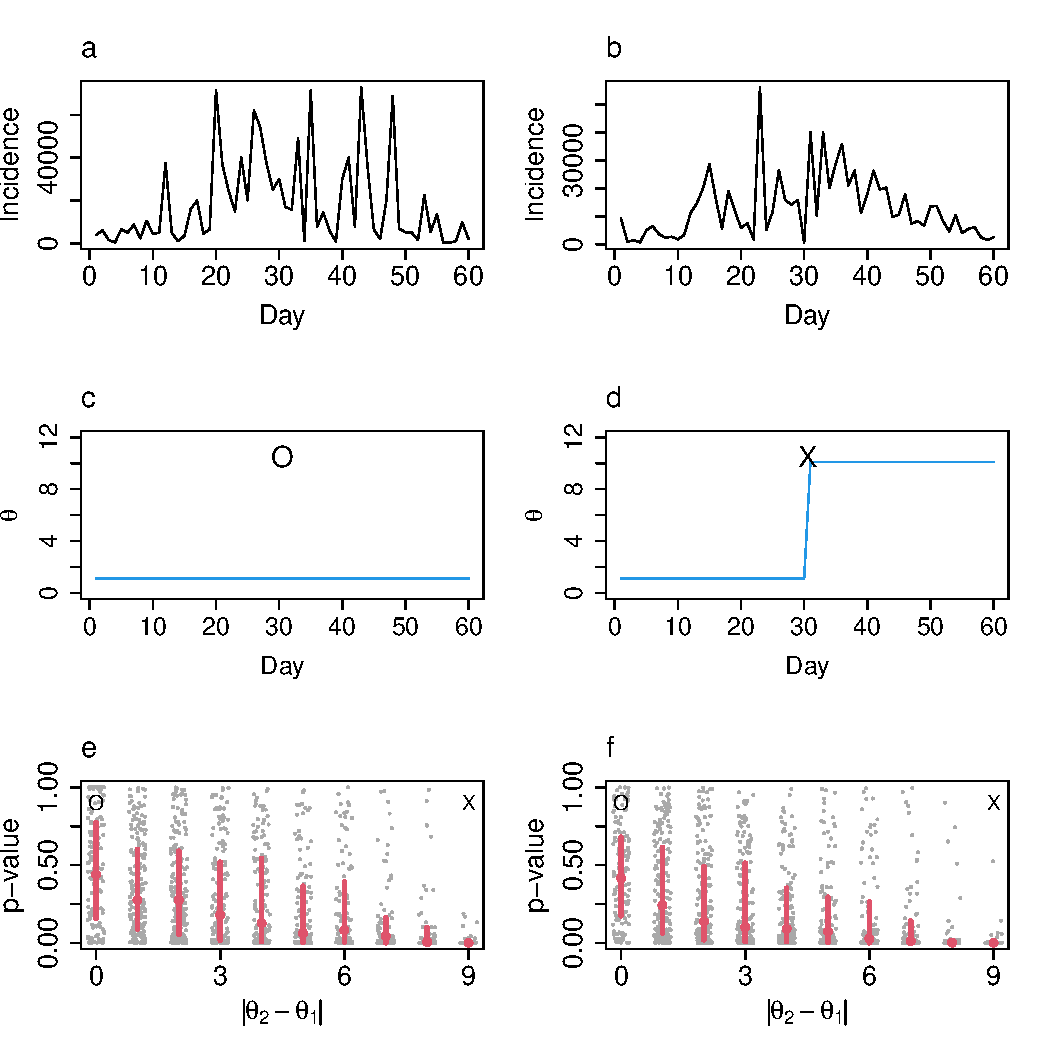
\includegraphics[width=0.6\textwidth]{fig1}
\caption{
Detecting dispersion changes in incidence time series in populations of different sizes. A: Simulated incidence when dispersion is constant. B: When dispersion changes during the epidemic. C:  D: Constant dispersion used in generation of above. E: Changing dispersion used in generation of above. F: Dispersion estimates from model fit to the above series. G: Performance of the method with simulated data that has different absolute differences in theta (horizontal axis of each pane) illustrates p-value distribution across different population sizes (each pane is one population size). O and X mark the null and alternative hypotheses indicated in panels D and E. 
 }
\label{fig1}
\end{figure}

Highly overdispersed incidence patterns were observed more frequently later in time series, consistent with more heterogeneity in transmission, susceptibility and reporting. 
The most dispersed category in Fig.2 (a) reaches its highest proportion near the end of the timeframe examined.
In addition, there are increases in dispersion around the peaks in incidence in the dataset (Fig. 2.(b,c)).
The evidence for a change in \begin{math}\theta\end{math} was observed across many counties (evidenced by concentration of low p-values around peak incidence) (Fig. 2 (d)).

\begin{figure}[!h]
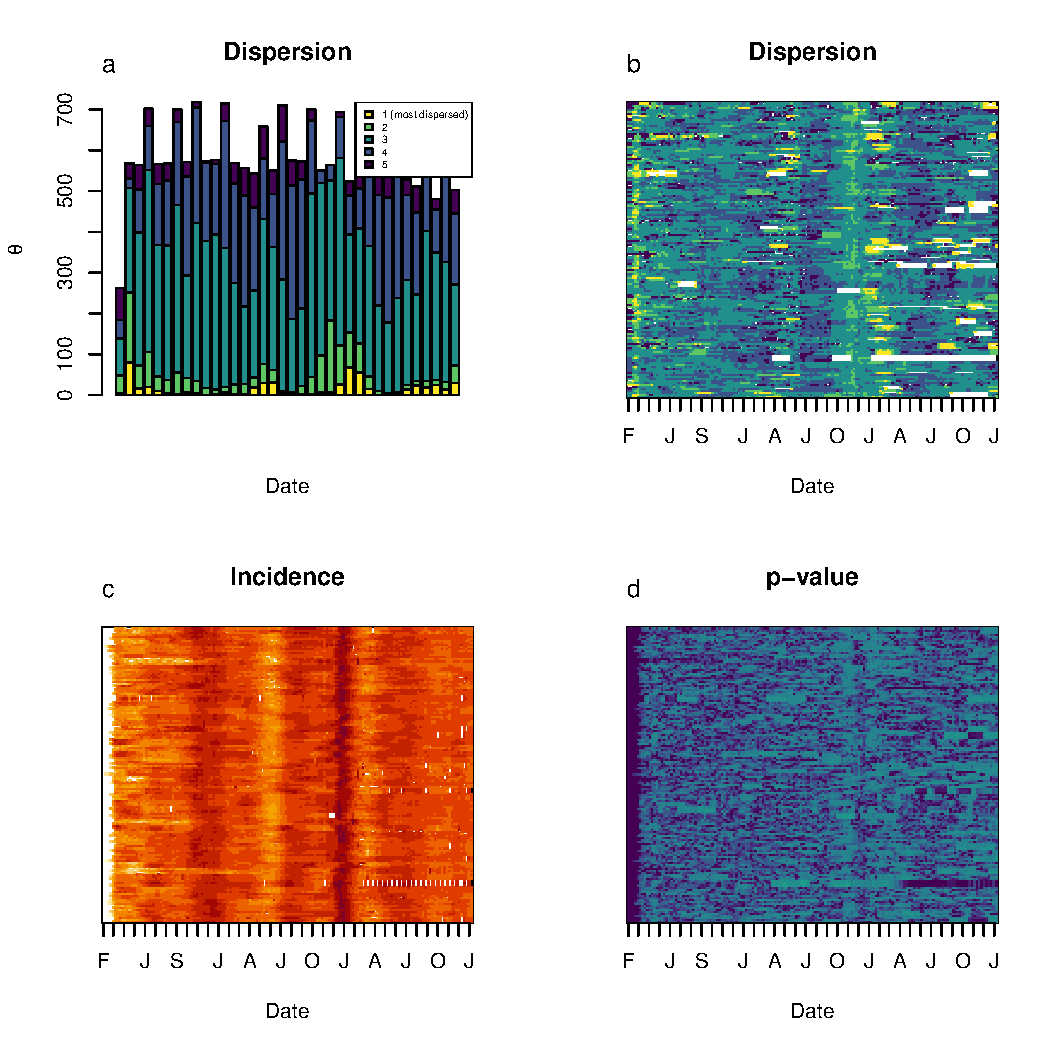
\includegraphics[width=0.6\textwidth]{fig2}
\caption{
Incidence and dispersion between 2020-01-04 and 2023-03-18 in large counties in the US. A: Binned log of the dispersion parameter over time. B: Log of the dispersion parameter over time as well as for each of the large counties (y-axis). C: Log incidence (new cases per individual) over time as well as for each of the large counties (y-axis). D: LRT p-values over time as well as for each of the large counties (y-axis).
}
\label{fig2}
\end{figure}

What makes a change in dispersion meaningful is how it affects variance-mean relationships. 

\begin{equation}
var = \mu + \mu^2/\theta  
\end{equation}

Raising variance relative to mean implies spatiotemporal "crowding" of cases (i.e. localized surges) which may necessitate more surge capacity in hospitals and testing centers. 
Additionally, it may indicate less diffuse epidemics that are potentially more subject to climate forcing \cite{dalziel_urbanization_2018}, or increased locally experienced mean density \cite{lloyd_mean_1967}. 

\section*{Discussion}
We presented an approach to quantify variability in epidemic time series that does not detect artifacts based on population size and incidence. 
Our method forms part of a larger push to investigate variability as an important attribute of epidemic time series.
Burst-tree decomposition of time series’ has also facilitated computation of a burst-size distribution for a series given a specified time window \cite{jo_burst-tree_2020}, allowing comparison of variability within one location over time. 
Similarly, spatial variation in superspreading potential has been investigated through e.g., risk maps of superspreading environments \cite{loo_identification_2021}.
Methods that use incidence time series are a crucial part of this research area due to the ease of obtaining incidence data, so the timing/geographical allocation of public health resources can be achieved with limited resources. 
Additionally, population-wide disease control approaches are often less effective than those which are targeted to individuals in high-transmission contexts \cite{lloyd-smith_superspreading_2005}, so models that incorporate transmission heterogeneity may catalyze the development of more efficient control strategies.
Our results imply that we can revise our understanding of case count dispersion: dispersion is high at unexpected times (near peak incidence).
Though large cities may be subject to more "smooth" epidemic dynamics, our contribution highlights the circumstances under which dynamics are less smooth in large counties. 
Previous research to evaluate bursty dynamics based on Influenza-like Illness (ILI) times series’ showed that epidemics in smaller communities are concentrated on narrower windows of the influenza season - the proportion of disease incidence that occurred in a given week was a metric of interest \cite{dalziel_urbanization_2018}. 
So, additional research is needed to understand the balance between burstiness of small communities and the potential impact of temporally changing dispersion in these areas.
Though some kinds of time dependence in the rate can cause autocorrelation, as can contagion (if it occurs outside of set periods), and heterogeneity (if an omitted variable is correlated in time) \cite{barron_analysis_1992}, our focus on dispersion makes sense because we are concerned with the clustering of cases from the point of view of an individual case, which is caused by these factors operating within a set period. Also, demographic structure (e.g., age structure) has the potential to affect temporal autocorrelation in transmission rate - the effects of age structure can be captured by a model that includes an infection rate that varies over time \cite{earn_dynamic_nodate}. 

\section*{Conclusion}

CO\textsubscript{2} Maecenas convallis mauris sit amet sem ultrices gravida. Etiam eget sapien nibh. Sed ac ipsum eget enim egestas ullamcorper nec euismod ligula. Curabitur fringilla pulvinar lectus consectetur pellentesque. Quisque augue sem, tincidunt sit amet feugiat eget, ullamcorper sed velit. 

Sed non aliquet felis. Lorem ipsum dolor sit amet, consectetur adipiscing elit. Mauris commodo justo ac dui pretium imperdiet. Sed suscipit iaculis mi at feugiat. Ut neque ipsum, luctus id lacus ut, laoreet scelerisque urna. Phasellus venenatis, tortor nec vestibulum mattis, massa tortor interdum felis, nec pellentesque metus tortor nec nisl. Ut ornare mauris tellus, vel dapibus arcu suscipit sed. Nam condimentum sem eget mollis euismod. Nullam dui urna, gravida venenatis dui et, tincidunt sodales ex. Nunc est dui, sodales sed mauris nec, auctor sagittis leo. Aliquam tincidunt, ex in facilisis elementum, libero lectus luctus est, non vulputate nisl augue at dolor. For more information, see \nameref{S1_Appendix}.

\section*{Supporting information}

% Include only the SI item label in the paragraph heading. Use the \nameref{label} command to cite SI items in the text.
\paragraph*{S1 Fig.}
\label{S1_Fig}
{\bf Bold the title sentence.} Add descriptive text after the title of the item (optional).

\paragraph*{S2 Fig.}
\label{S2_Fig}
{\bf Lorem ipsum.} Analytical approach: robust to population size changes.

\paragraph*{S1 File.}
\label{S1_File}
{\bf Lorem ipsum.}  Maecenas convallis mauris sit amet sem ultrices gravida. Etiam eget sapien nibh. Sed ac ipsum eget enim egestas ullamcorper nec euismod ligula. Curabitur fringilla pulvinar lectus consectetur pellentesque.

\paragraph*{S1 Video.}
\label{S1_Video}
{\bf Lorem ipsum.}  Maecenas convallis mauris sit amet sem ultrices gravida. Etiam eget sapien nibh. Sed ac ipsum eget enim egestas ullamcorper nec euismod ligula. Curabitur fringilla pulvinar lectus consectetur pellentesque.

\paragraph*{S1 Appendix.}
\label{S1_Appendix}
{\bf Lorem ipsum.} Maecenas convallis mauris sit amet sem ultrices gravida. Etiam eget sapien nibh. Sed ac ipsum eget enim egestas ullamcorper nec euismod ligula. Curabitur fringilla pulvinar lectus consectetur pellentesque.

\paragraph*{S1 Table.}
\label{S1_Table}
{\bf Lorem ipsum.} Maecenas convallis mauris sit amet sem ultrices gravida. Etiam eget sapien nibh. Sed ac ipsum eget enim egestas ullamcorper nec euismod ligula. Curabitur fringilla pulvinar lectus consectetur pellentesque.

\section*{Acknowledgments}
Cras egestas velit mauris, eu mollis turpis pellentesque sit amet. Interdum et malesuada fames ac ante ipsum primis in faucibus. Nam id pretium nisi. Sed ac quam id nisi malesuada congue. Sed interdum aliquet augue, at pellentesque quam rhoncus vitae.

\nolinenumbers

% Either type in your references using
% \begin{thebibliography}{}
% \bibitem{}
% Text
% \end{thebibliography}
%
% or
%
% Compile your BiBTeX database using our plos2015.bst
% style file and paste the contents of your .bbl file
% here. See http://journals.plos.org/plosone/s/latex for 
% step-by-step instructions.
% 
\bibliography{references}


\end{document}

